% Supplied November 5, 2026 in chat; acmart course template and metadata retained.
% Administrative details still require confirmation; see README.md.
\documentclass[sigconf,nonacm]{acmart}
\usepackage{graphicx}
\usepackage{booktabs}
% acmart already defines \comment; prefix only names that collide.
\usepackage[commandnameprefix=ifneeded]{changes}
\newcommand\vldbdoi{XX.XX/XXX.XX}
\newcommand\vldbpages{XXX--XXX}
\newcommand\vldbvolume{14}
\newcommand\vldbissue{1}
\newcommand\vldbyear{2020}
\newcommand\vldbauthors{\authors}
\newcommand\vldbtitle{\shorttitle}
\newcommand{\minihead}[1]{{\vspace{.45em}\noindent\textbf{#1.} }}
\newcommand\vldbavailabilityurl{}
\newcommand\vldbpagestyle{plain}
\emergencystretch=1.5em
\settopmatter{printacmref=false}
\begin{document}
\title{CS6400-A Project Milestone (Group 20): Replicating Low-Latency Transaction Scheduling}
\author{Brian Ok}
\affiliation{\institution{Georgia Institute of Technology}\city{Atlanta}\state{Georgia}\country{USA}}
\email{bok3@gatech.edu}
\author{Erin Tan}
\affiliation{\institution{Georgia Institute of Technology}\city{Atlanta}\state{Georgia}\country{USA}}
\email{etan61@gatech.edu}
\author{Erika Tay}
\affiliation{\institution{Georgia Institute of Technology}\city{Atlanta}\state{Georgia}\country{USA}}
\email{etay6@gatech.edu}
\begin{abstract}
We are implementing PreemptDB's transaction scheduling mechanisms in Silo.
At the November 5 midpoint evidence freeze, the independent request driver,
mixed New-Order/Payment/Q2 workload, Wait and Cooperative schedulers, context
state, batching, and starvation decisions have local functional evidence.
An experimental Linux-signal backend also passes continuation and state checks
inside restricted audited windows. A working Intel userspace-interrupt host
was not secured in time. Our midpoint therefore reports emulated x86-64 Linux
validation on a Mac: a matched two-policy smoke batch, separately labeled
signal pressure runs, and a controlled notification model. These establish
tested software behavior; native UINTR delivery, integration, and the paper's
three-policy performance comparison remain final-phase work.
\end{abstract}
\maketitle
\pagestyle{plain}
\raggedbottom

\section{Progress Check in}
\subsection{Implementation Progress}
Our target remains an independent Silo port of PreemptDB's scheduling design,
with Figure~10 as the first final experiment~\cite{huang2025preemptdb}.
We reuse Silo's engine and Masstree indexes~\cite{Tu2013Silo,silocode}; the
request driver, scheduler integration, Q2 adaptation, tests, and evidence tools
are project additions. Inspecting the authors' implementation~\cite{preemptcode}
does not constitute an author-artifact experiment; none is included here.

\minihead{Completed locally}
An independent producer schedules short requests without waiting for workers.
Bounded fixed-routing queues retain rejected and cancelled work. Request IDs,
inputs and generation timestamps survive retries. The mixed workload uses
real New-Order and Payment adapters plus the read-only snapshot
\texttt{q2\_min\_stock\_v1} port, with deterministic minimum-stock checksums.
Wait dispatches high work at transaction boundaries; Cooperative can pause Q2
at audited completed reads. Two guarded contexts preserve low transaction
storage and its snapshot across intervening high work. Nested protection
defers service through unsafe regions and write cleanup.

The software notification model covers delayed, duplicate, coalesced and
spurious hints separately from admitted requests. Batched admission/drain and
starvation budget decisions pass controlled and real-Q2 cases. The opt-in
\texttt{linux-signal} backend captures/restores actual kernel signal frames
inside bounded assembly windows. Queue fallbacks remain separately counted.
This is asynchronous capture within the documented windows, not arbitrary
interruption throughout Silo or libc. Table~\ref{tab:validation} summarizes
the local acceptance evidence.

\minihead{In progress and not yet started}
The UINTR sender/receiver kit is buildable, but native I12 delivery and
receiver resumption have not passed. Native interrupt context switching,
Preemptive Silo integration, hardware batching/return races, and native
starvation validation remain I13--I16. Complete native integrated validation
(I17), the matched native experiment (I18), and the final report remain open.
No local signal/model pass changes those native statuses.

\subsection{Division of Work}
The shared roadmap assigns Erin hardware qualification and switching, Brian
engine/context protection and scheduler integration, and Erika the driver,
workload and experiment pipeline, with joint validation and reporting.
MAC-01--MAC-10 handoff entries record Erin's local evidence sessions. These
are the recorded responsibilities and checkout results; individual member
contribution sign-off remains pending. We do not infer personal authorship
or hours from aggregate test logs.

\subsection{Progress Assessment and Remaining Work}
The supplied planning record promised a working interrupt host, two contexts,
context-local state, and Wait/Cooperative measurements at the milestone.
The software components have substantial local evidence, but the host goal
was missed. This is partial progress toward the original replication, not
a completed hardware replication. Separate teammate-Mac reproductions were
not recorded. The supplied milestone draft is now available as the template;
the verbatim original proposal plan and any separate course page limit/rubric
were not supplied for exact comparison.

The midpoint and final submission deadlines and group submitter are still
unconfirmed. The following dates are proposed decision checkpoints as of
November~5; they are not asserted course deadlines.
\begin{itemize}\itemsep0pt
\item \textbf{November 6:} confirm Canvas deadlines, submitter and rubric;
  review this package and map the remaining milestones onto the final date.
\item \textbf{November 8:} record a candidate host access decision. Proceed
  only after CPUID, approved kernel/interface, sender/receiver delivery and
  continuation pass. If unavailable, take the evidence to course staff while
  continuing local work. No provider or quota approval is assumed.
\item \textbf{After qualification:} finish native I13 state preservation,
  I14 short-during-Q2 service/resumption, and I15--I17 batching, fairness,
  conflicts, cleanup and integrated correctness before performance runs.
\item \textbf{Final minus 7 days:} freeze validated code and run the matched
  pilot/main comparison. \textbf{Final minus 3 days:} freeze results and
  complete analysis/report. Rebase these relative gates once the final date
  is confirmed; reduce the matrix and consult staff if the gates cannot fit.
\end{itemize}

\section{Preliminary Validation and Results}
\subsection{Environment and Evidence Freeze}
Saved local runs used an Apple M5 Pro with a Colima/QEMU x86-64 Linux guest,
Ubuntu 22.04.5, GCC 11.4 and glibc 2.35, with two emulated vCPUs and inherited
process affinity. Workers/sender were not individually pinned. The disposable
engine builds used the archived GCC compatibility patch and \texttt{-O1};
the Mac checkout was not patched. Emulation timings are preliminary and do
not measure native UINTR cost or establish the paper's performance claims.

The package freezes source \texttt{7319ba6} (full hash in the manifest), with
Masstree \texttt{1150824}. Historical runs retain their own base revision,
source overlay, environment, binary hashes, commands and configuration;
they were not all rerun at the freeze. Evidence IDs below resolve through the
package evidence index. MAC-11 reruns saved-trace verifiers and analysis,
not the engine or hardware tests. All old failure records are retained.

\begin{table*}[t]
\caption{Component validation actually archived. Repetitions are executions of
the same cases, not independent correctness proofs. E09/E10 overlap in regression
coverage and must not be added as disjoint totals.}
\label{tab:validation}
\small
\begin{tabular}{p{.18\textwidth}p{.54\textwidth}p{.20\textwidth}}
\toprule
Component / evidence & Observed result & Scope / remaining check \\
\midrule
Build, context / E01--E05 & Three engine targets built; both engine tests and driver passed.
Voluntary ABI tests passed one million round trips per build; E04 trap fixtures passed
256 returns and detected deliberate corruption. & Emulated Linux software checks;
trap/voluntary paths do not validate UINTR. \\
Signal state / E09 & 69 state cases (23 normal, 23 R12-corruption, 23 XMM0-corruption);
1,518 captures/returns, with 1,382 arithmetic-interior captures in normal runs.
Negative controls detected corruption. & Restricted windows; legacy x87/MXCSR/XMM
state; AVX/AMX/CET unvalidated. \\
Batching / E09 & 11 standalone cases per build/repeat; nine real Q2 transition cases
retained checksum across 36 writes and 15 actual captures/resumptions. & Debug,
optimized, UBSan and 20 optimized repeats; hardware races pending. \\
Budget / E09 & Four standalone cases per execution; real Q2 cases committed seven Q2s
and 22 high writes. Exact threshold, recovery, reset, retries and drain checked. &
Whole-high-request charging; decisions between requests, not a strict CPU cap. \\
Cleanup / E09, E10 & 53 real failed-write rollback/cleanup probes while Q2 was paused;
stored values and protection state checked. & Separate from driver-scripted retries. \\
Notification model / E10 & 419 controlled blocks / 2,848 terminal records and 822 events /
94 schedules reconciled, including separate signal engine regressions. Two new real Q2
schedules preserved the same-attempt checksum across four writes and two voluntary resumes. &
Model-only paths have zero real handlers/captures; close requires quiescence. \\
Tooling / E10 & Both Linux driver builds and all 15 tool tests passed; Mac transport
normal/ASan/UBSan, Wait driver and 15 tool tests passed. & No fresh pressure or full upstream
Silo suite in E10. \\
Hardware / E03 & Standalone kit built; guest and both pinned vCPUs returned
\texttt{UINTR=0}; delivery executable exited 77 at guard. & Prepared, not delivered;
qualify another host. \\
\bottomrule
\end{tabular}
\end{table*}

\subsection{Matched Wait/Cooperative Smoke (E05)}
Eight actual runs used one/two workers and matching warehouse counts, two
repetitions with varied policy order, seed 1, one-second warmup and measurement,
30-second drain, and four shorts per worker every 100\,ms. Global/local high
queue capacities were four per worker; Cooperative used 64 completed reads.
Matching short inputs and deadlines and common Q2 input prefixes were verified.
Every measurement arrival committed: 7,910 total, including 432 shorts and
7,478 Q2s, with zero aborts, rejection, cancellation or missing terminal records.
Cooperative made 40 handoffs and served 160 shorts while Q2 was paused; Wait
had zero same-worker overlap. Table~\ref{tab:smoke} reports each run, avoiding
an average of per-run percentiles.

\begin{table*}[t]
\caption{E05 measurement cohorts, including drain commits. W/R denotes workers/repetition.
Window counts commits before cutoff; handoffs are mid-Q2. These are functional smoke
counts, not native throughput comparisons.}
\label{tab:smoke}
\centering\small\begin{tabular}{llrrrrrr}
\toprule
Policy & W/R & Commits & Short & Q2 & Window & Drain & Handoffs \\
\midrule
Wait & 1/1 & 756 & 36 & 720 & 754 & 2 & 0 \\
Coop. & 1/1 & 706 & 36 & 670 & 705 & 1 & 7 \\
Wait & 2/1 & 1162 & 72 & 1090 & 1158 & 4 & 0 \\
Coop. & 2/1 & 1260 & 72 & 1188 & 1256 & 4 & 11 \\
Wait & 1/2 & 745 & 36 & 709 & 744 & 1 & 0 \\
Coop. & 1/2 & 726 & 36 & 690 & 725 & 1 & 7 \\
Wait & 2/2 & 1327 & 72 & 1255 & 1324 & 3 & 0 \\
Coop. & 2/2 & 1228 & 72 & 1156 & 1225 & 3 & 15 \\
\bottomrule
\end{tabular}

\end{table*}

Table~\ref{tab:latency} shows the first one-worker repetition to illustrate
the verified latency pipeline. The package retains all 24 per-type rows,
including queue delay, throughput, p50/p90/p99/p99.9, sample counts and outcomes.
Latency is finish minus actual generation time, with original time retained
across retries; scheduled latency is retained separately. Quantiles use nearest
rank over committed requests including drain. Throughput uses only commits
before cutoff divided by the measurement duration. Small-sample p99.9 values
are exposed and flagged, not used as evidence of tail improvement.
The default 10,000-read smoke in E02 reached zero checkpoints: measured Q2
eligible reads were only 843--2,363 per query. Thus interval 64 is a functional
test setting, not equivalence to the paper's configuration.

\begin{table*}[t]
\caption{E05 one worker, repetition 1, end-to-end latency in microseconds.
All p99.9 entries (*) have fewer than 1,000 observations and are low-sample
diagnostics. No native performance conclusion is drawn.}
\label{tab:latency}
\centering\small\begin{tabular}{llrrrrr}
\toprule
Policy & Type & $n$ & p50 & p90 & p99 & p99.9* \\
\midrule
Wait & NewOrder & 20 & 684.8 & 1701.5 & 2009.4 & 2009.4 \\
Wait & Payment & 16 & 614.8 & 1696.5 & 1785.4 & 1785.4 \\
Wait & Q2 & 720 & 1650.5 & 2600.2 & 3343.9 & 4551.6 \\
Coop. & NewOrder & 20 & 437.9 & 768.8 & 1368.6 & 1368.6 \\
Coop. & Payment & 16 & 434.9 & 654.8 & 1090.7 & 1090.7 \\
Coop. & Q2 & 670 & 1915.4 & 2978.1 & 4164.8 & 5082.5 \\
\bottomrule
\end{tabular}

\end{table*}

\subsection{Signal Pressure and Progress (E09)}
These four separate functional runs used the same signal binary, one/two
workers, seed 1, no warmup, three seconds measurement, ten seconds drain and
four shorts per worker every 1\,ms, at 25\% and 100\% budgets. They are not
matched to the sparse E05 smoke and cannot supply its third policy.
Every one of 71,976 short arrivals reconciles to 39,749 commits or 32,227
queue-full rejections (Figure~\ref{fig:pressure}); none was cancelled or missing.
Q2 committed 6,577 times with recorded checksums and positive measured
low-context service. That service is elapsed local monotonic time, not CPU time.

The runs recorded 8,465 actual captures versus 14,065 total mid-low handoffs;
5,600 handoffs used voluntary fallback. Only captures support asynchronous
switch claims. Restrictive 25\% recorded 7,315 forced low returns and 518
admission blocks; 100\% recorded neither. Table~\ref{tab:pressure} retains each
configuration. Pressure produced zero real short conflicts; retry/rollback
coverage comes from controlled/engine checks. Rejections are not successful
short requests and are excluded from committed-latency samples.

\begin{table*}[t]
\caption{E09 signal pressure accounting. Return/block are budget decisions;
capture is actual signal-frame capture. One repetition per configuration.}
\label{tab:pressure}
\centering\small\begin{tabular}{rrrrrrrr}
\toprule
Budget & W & Q2 & Short & Reject & Capture & Return & Block \\
\midrule
25\% & 1 & 1181 & 7693 & 4303 & 1649 & 3870 & 283 \\
25\% & 2 & 1826 & 10813 & 13179 & 2661 & 3445 & 235 \\
100\% & 1 & 1415 & 8960 & 3036 & 1423 & 0 & 0 \\
100\% & 2 & 2155 & 12283 & 11709 & 2732 & 0 & 0 \\
\bottomrule
\end{tabular}

\end{table*}
\begin{figure*}[t]
\centering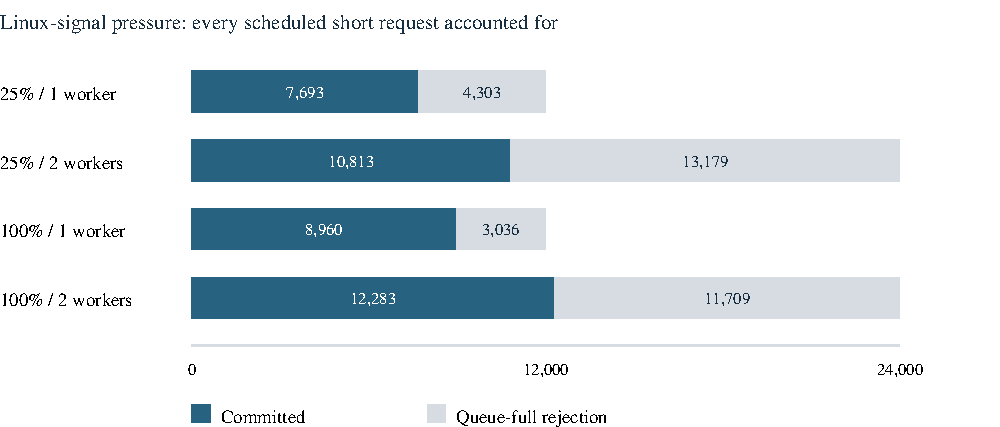
\includegraphics[width=.85\textwidth]{generated/pressure-outcomes.pdf}
\caption{Emulated Linux signal-only pressure outcomes, E09. Bars include rejection;
no slow or rejected requests are silently counted as commits. Counts regenerate
from archived terminal records.}
\Description{Four stacked horizontal bars show committed and queue-full-rejected short requests
for 25 and 100 percent budgets with one and two workers. Every arrival has an outcome.}
\label{fig:pressure}
\end{figure*}

\subsection{Failures, Replay and Interpretation}
E05 unintentionally restarted an old container entrypoint; that extra process
was paused before its validation and excluded. E08 stopped after a malformed
analysis invocation; recovery collected/analyzed remaining cases, and the
entire corrected script was not rerun. E09 retained staging, classification,
compile and controlled-clock reset failures. The full validation passed,
followed by a passing focused fixture rebuild; the full script was not
repeated after fixture-only improvements. Runtime/pressure-binary continuity
was checked. E10 retained a dependency-metadata setup failure and an incorrect
two-publication fixture assumption; the entire corrected script then passed.
The first MAC-11 replay hit a Mac temporary-path alias check; resolving the
temporary root fixed the packaging check and the full replay then passed.

The frozen package includes these failed attempts, not just final passes.
MAC-11 independently replays E09 and E10 raw records and E05 metrics; saved
reconciliation JSON and all four E05 CSV/report files regenerate identically.
The same-attempt Q2 fixtures use checksum \texttt{12860241382490130518}.
They support tested continuation through intervening committed writes; they
are not a proof of correctness under all schedules. No native UINTR test,
new engine benchmark, native three-policy comparison, or teammate-Mac run
was performed for this report. Historical PACE stock measurements are retained
in the source evidence but are not pooled into the local midpoint results.

\section{Evolving Methodology}
\subsection{Updated Plan}
Changes below use the supplied draft's \texttt{changes} notation. The original
proposal's full Replication Plan was not supplied, so exact unchanged text and
complete word-level differences against it still require group verification.
\begin{itemize}\itemsep2pt
\item \textbf{Claim.} The paper's reported 88--96\% improvement is over
\deleted{cooperative yield}\added{Wait; this is an external result, not a
required outcome of the Silo port}~\cite{huang2025preemptdb}.
\item \textbf{Setup.} \added{The midpoint uses saved Mac/emulated-Linux evidence
because a working UINTR host was not secured. The guest and prior AWS VM report
UINTR=0; these results apply to those environments. PACE has no usable interface
available to the team. Qualify each alternative independently before claiming access.}
\item \textbf{Host fallbacks.} \added{Pursue an approved Intel cloud or physical
host; verify exposure, interface permission and actual delivery. The authors'
artifact may provide a separately labeled reference run on a qualified host.
If the November 8 access checkpoint fails, consult staff; retain native UINTR
as the final objective unless a scope change is approved.}
\item \textbf{Workload.} \added{Retain the documented q2\_min\_stock\_v1 Silo
projection and checksum oracle. Measure reads/runtime on the eventual native
host before setting scale and intervals; no unsupported 140-microsecond estimate
or claimed millisecond runtime is used. Record all departures from the paper.}
\item \textbf{Cooperative.} Yield every \deleted{10,000}\added{$N$ completed
record reads, with $N=64$ for the archived smoke. Test the paper's 10,000 on the
final workload and report observed checkpoints rather than assuming they occur.}
\item \textbf{Driver/measurement.} \added{Use open-loop arrivals and explicit
outcomes. Keep per-run quantiles and counts; never average quantiles. Any pooled
summary must identify its exact cohorts. Retain low-sample tail flags, retries,
rejections, cancellation and cutoff/drain accounting. Match all policies on
one qualified host before the native comparison.}
\item \textbf{Implementation order.} \added{Voluntary contexts and protected
regions precede native delivery/switching. The glibc voluntary ABI tests do
not validate interrupt-time state. Native I12--I17 acceptance gates remain mandatory.}
\item \textbf{Scheduler substitute.} \deleted{The Linux-signal backend is not
yet built.}\added{It is locally implemented and tested for restricted audited
windows. Signal batching/starvation repetitions are complete locally. Model
events use checkpoint service and remain separate from real handlers/captures;
neither substitutes for native UINTR delivery or native performance.}
\item \textbf{Final experiments.} \added{Target Figure 10-style matched Wait,
Cooperative and native Preemptive runs after correctness gates, then confirm
additional coverage against the final rubric. Record host limits versus the
paper's 16-worker setup, queue capacities, intervals, duration and core placement.
Defer adaptive thresholds, architecture and distributed extensions.}
\end{itemize}

\subsection{Justification of Changes}
Unresolved machine access caused the local midpoint/native final split.
The 10,000-read zero-checkpoint result motivates testing smaller intervals
without treating them as paper-equivalent. The restricted signal contract
provides executable continuation tests while preserving the distinction from
hardware interrupts. Overload rejections and sparse short samples require
explicit outcome/sample reporting. Silo's transaction and data layout differ
from the original engine, so effects must be measured within Silo rather than
inferred from the published result. The proposed dated gates protect time for
native validation and reporting once the actual deadline is confirmed.

\subsection{Response to Proposal Feedback}
We investigated PACE and an AWS VM but did not secure a usable UINTR host;
the VM and emulated guest reported \texttt{UINTR=0}, while PACE offers no usable
interface to our team. We prepared a standalone qualification/delivery kit and
propose a November 8 approved-host decision, followed by staff consultation if
access is still unresolved; planned cloud access is not reported as acquired.

\section{Potential Risks and Mitigation}
\minihead{Locally addressed}
The saved tests reduce uncertainty about the implemented queue accounting,
voluntary state isolation, restricted signal continuation, and tested budget
decisions. They do not resolve native delivery or general concurrency correctness.
Two principal risks remain:
\begin{enumerate}\itemsep2pt
\item \textbf{Host qualification.} If no approved host passes actual delivery
by the proposed November 8 checkpoint, Erin will take capability/interface
evidence to course staff and seek a qualified alternative or an explicit scope
decision. A compatible CPU model, cloud plan or pending quota request is not
a working UINTR interface.
\item \textbf{Unfinished native integration.} If I13--I17 expose state corruption,
cleanup failures, missing requests or no committed Q2 progress, Brian and Erin
will isolate the failing mechanism on tiny fixtures before performance runs.
Erika will preserve matched baselines and failure traces. At final minus 7 days,
reduce sensitivity work and escalate any core blocker rather than measure
unvalidated code or silently change transaction semantics.
\end{enumerate}

\bibliographystyle{ACM-Reference-Format}
\bibliography{ref}
\end{document}
